\documentclass[a4paper]{article}
\usepackage[a4paper, margin=4cm]{geometry}
\usepackage{amsmath}
\usepackage{amssymb}
\usepackage{xcolor}
\usepackage{amsthm}
\usepackage{dsfont}
\usepackage{graphicx}
\usepackage{hyperref}
\usepackage{datetime}
\usepackage{outlines}
\usepackage{float}
\usepackage{booktabs}
\usepackage{enumitem}

% link coloring
%\hypersetup{
%    colorlinks,
%    linkcolor={red!80!black},
%    citecolor={green!60!black},
%    urlcolor={blue!80!black}
%}

% concatenation symbol (c.f. ++ in Haskell)
\newcommand\mdoubleplus{\mathbin{+\mkern-10mu+}}

% end of proof symbol
\newcommand{\newmarkedtheorem}[1]{%
  \newenvironment{#1}
    {\pushQED{\qed}\csname inner@#1\endcsname}
    {\popQED\csname endinner@#1\endcsname}%
  \newtheorem{inner@#1}%
}

\theoremstyle{definition}
%\newtheorem{eg}{Example}[section]
\newmarkedtheorem{eg}{Example}[section]
\newtheorem{observation}{Observation}[section]
\newtheorem{define}{Definition}[section]
\theoremstyle{plain}
\newtheorem{proposition}{Proposition}
\newtheorem{lemma}{Lemma}
\newtheorem{corollary}{Corollary}
\newtheorem{theorem}{Theorem}[section]
\newtheorem{assump}{Assumption}[section]
\newtheorem{remark}{Remark}[section]

\newdateformat{monthyeardate}{\monthname[\THEMONTH] \THEYEAR}

\author{Jeroen van Riel}
\date{\monthyeardate\today}
\title{}

\begin{document}

%\section*{Research Plan}

\subsection*{Introduction}

% possibly add some motivation

Various models and systems have been proposed in the literature for the problem
of coordinating autonomous vehicles through urban road networks. Previous works
vary considerably in the types of communication model, which can be roughly
categorized in distributed approaches, where groups of vehicles coordinate
trajectories together, and centralized approaches, where individual vehicles
receive instructions from a central controller.
%
We are mainly interested in the latter type, so we will discuss some examples
from the literature in the next section. For a more complete overview of previous
works, we refer to the survey~\cite{khayatianSurveyIntersectionManagement2020}.

% introduce stylized model

In its most pure form, the coordination of autonomous vehicles through a road
network with intersections may be regarded as a high-dimensional optimal control
problem. Most previous works with this perspective use the a simple
one-dimensional vehicle model known as the double integrator~\cite{raoNaiveControlDouble2001} in optimal
control literature. Imagine that some central coordinator controls the
acceleration of each individual vehicle.
% route, speed control, objective
After a vehicle arrives to the network, it follows a predetermined route and
leaves again. The goal is to control the trajectory of each vehicle in the
network while avoiding collisions and optimizing some global measure of
efficiency. A natural measure of efficiency that is commonly used in literature
is total delay experienced by all vehicles. However, it might be desirable to
also penalize acceleration as a proxy for energy consumption.
% online vs offline
When all vehicle arrival times are known in advance, we may assume that
trajectories can be computed without any prior interaction with the system, so
we refer to this setting as \textit{offline trajectory optimization}.

% crossing order
A key issue for the coordinator is to decide the \textit{order of crossing} at
intersections, which is precisely what makes the optimization problem non-convex
and thus hard to solve with standard methods. Under some assumptions, the
problem can be shown to decompose in a combinatorial problem to determine a
\textit{crossing time schedule} --- indicating when vehicles cross the intersections
along their route --- and an optimal control problem to find trajectories that
match these crossing times. We propose to address the scheduling part by
applying recent machine learning methods for combinatorial optimization.

%\begin{figure}
%  \centering
%  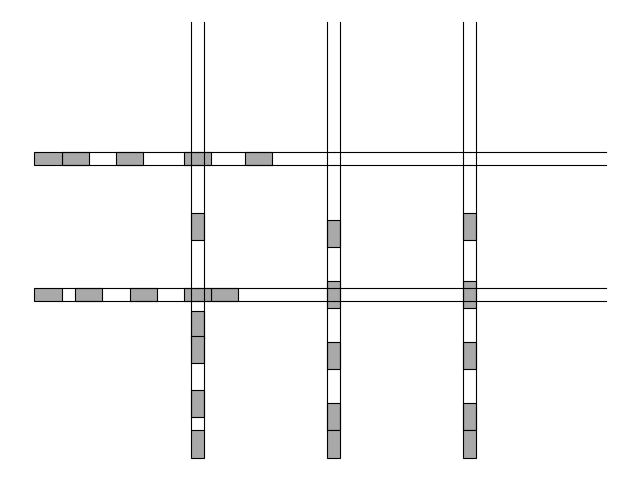
\includegraphics[width=0.6\textwidth]{figures/state_example.png}
%  \caption{Illustration of some grid-like network of intersections with vehicles
%    drawn as grey rectangles. There are five vehicle routes: two from east to
%    west and three from south to north. Turning at intersections is not
%    allowed.}\label{fig:network_illustration}
%\end{figure}

\subsection*{Autonomous intersection control}

A good example of an early centralized approach is the ``Autonomous Intersection
Management'' (AIM) paper~\cite{dresnerMultiagentApproachAutonomous2008}, which
is based on a reservation scheme. The conflict zone is modeled by a grid of
cells. Vehicles that want to cross the intersection send a request to the
central controller to occupy the cells containing its trajectory for a certain
amount of time. The central controller then decides to grant or deny these
requests based on previous granted requests, in order to facilitate
collision-free trajectories. If a request is denied, the vehicle slows down and
attempts to obtain a new reservation after some timeout.

%\begin{figure}[t]
%  \centering
%  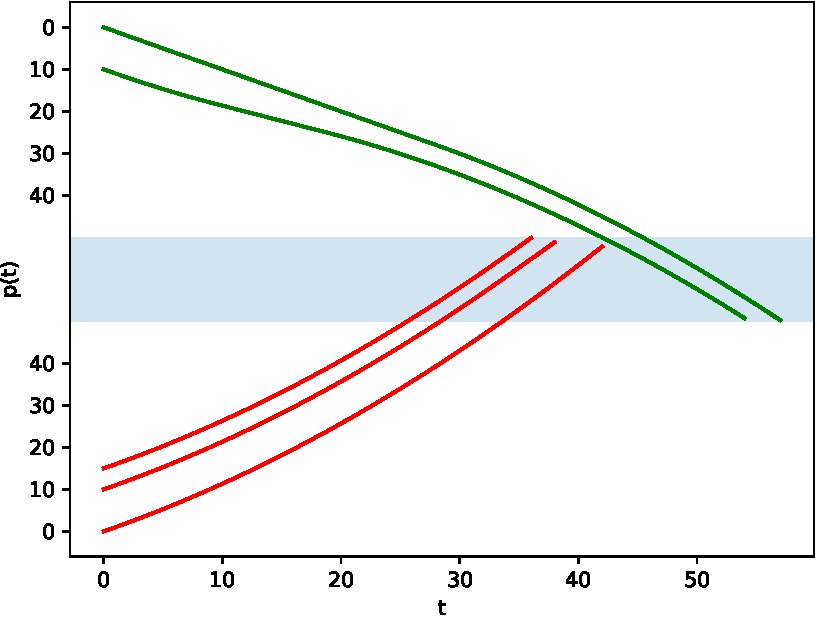
\includegraphics[width=0.8\textwidth]{figures/direct_transcription_example.pdf}
%  \caption{Example of optimal trajectories approaching a single intersection,
%    obtained using a direct transcription method. The objective that was used
%    penalizes the absolute value of acceleration. The y-axis is split such that
%    each part corresponds to one of the two approaching lanes with the
%    corresponding trajectories drawn in separate colors. The intersection area
%    is shown as a shaded region. To improve clarity of the figure, trajectories
%    have been truncated after they leave the intersection.}
%\end{figure}

% direct transcription
Optimal control problems can be approached in an end-to-end fashion by
\textit{direct transcription} to an equivalent mixed-integer optimization
problem, which can be solved using off-the-shelf solvers (e.g., SCIP~\cite{BolusaniEtal2024OO} or
Gurobi~\cite{gurobi}). Such methods can be used to compute optimal trajectories up to any
precision, by choosing a fine enough time discretization. However, it is exactly
this time discretization that causes prohibitive growth of the number of
variables with respect to the size of the network and the number of vehicles, so
this method is only really useful for toy problems.
%
Therefore, approximation schemes have been studied in previous works. A common
observation is that the optimization problem may be thought of as two coupled
optimization problems, where the upper-level problem is to determine when and in
which order vehicles enter and exit each intersection on their route. The
lower-level problem is to find optimal trajectories that match these time slots.
% Hult et al. (offline single intersection with energy objective)
% "An approximate solution to the optimal coordination problem for autonomous
% vehicles at intersections"
The approximation method in~\cite{hultApproximateSolutionOptimal2015} is based
on this bilevel decomposition and considers an quadratic objective involving
velocity as a proxy for energy. The first stage optimizes a schedule of vehicle
crossing times. It uses approximations of each vehicle's contribution to the
total objective, as a function of its crossing time. Next, for each vehicle, the
second stage computes an optimal trajectory that satisfies the crossing time
schedule by solving a quadratic program. This approach has been shown to reduce
running times significantly. Unfortunately, this study is limited to a single
intersection and it is assumed that each lane approaching the intersection
contains exactly one vehicle.
% Zhao et al. (bilevel programming model)
The paper~\cite{zhaoBilevelProgrammingModel2021} proposes a trajectory
optimization scheme for a single intersection, also based on the bilevel
decomposition. The lower-level problem is employed to maximize the speed at
which vehicles enter the intersection. Both levels are solved in an alternating
fashion, each time updating the constraints of the other problem based on the
current solution.
% bubbles paper
The optimization scheme
in~\cite{tallapragadaHierarchicaldistributedOptimizedCoordination2017} deals
explicitly with the complexity of the crossing order decisions by defining
groups of consecutive vehicles on the same lane. The first step is to group
vehicles into these so-called ``bubbles''. All vehicles in a bubble are required
to cross the intersection together, while maintaining feasibility with respect
to safe trajectories. Next, crossing times are assigned to bubbles while
avoiding collisions. Based on this schedule, a local vehicular control
method~\cite{tallapragadaDistributedControlVehicle2017} is used that guarantees
safety to reach the assigned crossing times.

\subsection*{Job-shop scheduling}

Optimizing the crossing time schedule in a network of intersections is very
similar to the classical Job-Shop Scheduling Problem (JSSP). Therefore, we
briefly discuss this class of models such that we can use the related
terminology and notation in the following.
%
The classical JSSP problem considers a set of $n$ jobs that must be assigned to
non-overlapping time slots on a set of $m$ machines. Each job $i$ has a set of
$n_{i}$ operations $O_{i1}, \dots, O_{in_{i}}$ that need to be executed in this
order. Each operation $O_{ij}$ requires $p_{ij}$ processing time on machine
$M_{ij}$. Each machine can process at most one operation and early preemption is
not allowed. The task of the scheduler is to determine a valid schedule of start
times $y_{ij}$ for each operation, while minimizing some objective function. Let
$C_{ij} = y_{ij} + p_{ij}$ denote the \textit{completion time} of operation $O_{ij}$.
Common optimization objectives are a function of these completion times, e.g.,
minimizing the total completion time among operations or minimizing the maximum
completion time, also known as the \textit{makespan}. Objectives that are a
non-decreasing function of completion times are called \textit{regular}.

% disjunctive graph
A commonly used representation of JSSP instances is the \textit{disjunctive
  graph} , with vertices $\{ O_{ik} : 1 \leq i \leq n, 1 \leq k \leq n_{i} \}$
corresponding all the operations. The set of \textit{conjunctive arcs} encodes
all the precedence constraints $O_{i,k} \rightarrow O_{i,k+1} $ among each job's
operations. The set of \textit{disjunctive edges} consists of undirected edges
between each pair of operations from distinct jobs that need to be processed on
the same machine, effectively encoding all such \textit{conflicts}. Each valid
schedule induces an ordering of operations on machines that is encoded by fixing
the direction of each disjunctive edge such that we obtain a direct acyclic
graph.

\subsection*{Neural combinatorial optimization}

% maybe discuss traditional epsilon-approximation schemes?
% argue that it takes a lot of expert knowledge about the problem structure to design these

This section will introduce the idea of applying a Machine Learning (ML) perspective
on Combinatorial Optimization (CO) problems, which has recently gained a lot of
attention. One of the key ideas in this line of research is to treat problem
instances as data points and to use machine learning methods to approximately
map them to corresponding optimal
solutions~\cite{bengioMachineLearningCombinatorial2020}.
% learning assumptions:
% supervised learning (expert labels) vs reinforcement learning (experience)
It is very natural to see the sequential decision-making process of any
optimization algorithm in terms of the Markov Decision Process (MDP) framework,
where the environment corresponds to the internal state of the algorithm. From
this perspective, two main learning regimes can be distinguished.
% imitiation learning
Methods like those based on the branch-and-bound framework are
often computationally too expensive for practical purposes, so \textit{learning
  to imitate} the decisions taken in these exact algorithms might provide us
with fast approximations. In this approach, the ML model's performance is
measured in terms of how similar the produced decisions are to the
demonstrations provided by the expert.
% reinforcement learning
On the other hand, some problems do not even enable exact methods, so it is
interesting to study solution methods that \textit{learn from experience}. An
interesting feature of this kind of approach is that it enables us to implicitly
exploit the hidden structure of the problems we want to solve.

% neural combinatorial optimization
Because neural networks are commonly used as encoder in these ML models for CO,
we will refer to this new field as \textit{Neural Combinatorial Optimization} (NCO).
%
A wide range of classical combinatorial optimization problems has already been
considered in this framework, so we briefly discuss the taxonomy used in the
survey~\cite{mazyavkinaReinforcementLearningCombinatorial2020}.
% principal vs. joint approach
One distinguishing feature is whether existing off-the-shelf solvers are used or
not. On the one hand, \textit{principal} methods are based on a parameterized
algorithm that is tuned to directly map instances to solutions, while
\textit{joint} methods integrate with existing off-the-shelf solvers in some
way. An illustrative example of the latter category are the use of ML models for
the branching heuristic or the selection of cutting planes in branch-and-cut
algorithms~\cite{tangReinforcementLearningInteger2020}.
% principal - construction vs. improvement (guided search)
The class of principal methods can be further divided into \textit{construction}
heuristics, which produce complete solutions by repeatedly extending partial
solutions, and \textit{improvement} heuristics, which aim at iteratively improving the
current solution with some tunable search procedure.


% learning algorithms:
% REINFOCE with baseline
% Fitting the neural mapping is often done using policy gradient methods (with
% baseline), e.g., with the classical REINFORCE algorithm.

% constraints in differentiable models

A major challenge in NCO is constraint
satisfaction. For example, solutions produced by constructive neural policies
need to satisfy the constraints of the original combinatorial problem.
Therefore, an important question is how to enforce these constraints. To this
end, neural network architectures have been designed whose outputs satisfy some
kind of constraint, for example being a permutation of the
input~\cite{vinyalsPointerNetworks2017a}. Constraints can also be enforced by
the factorization of the mapping into repeated application of some policy. For
example, in methods for TSP, a policy is defined that repeatedly selects the
next node to visit. The constraint that nodes may be only visited once can be
easily enforced by ignoring the visited nodes and taking the argmax among the
model's probabilities for unvisited nodes.


% encoders:
% standard multilayer perceptron networks are not suited to encode order
% pointer networks
% graph neural networks


% examples for job-shop scheduling
Various NCO methods have already been studied for JSSP with makespan objective,
of which we now highlight some works that illustrate some of the above classes
of methods. A lot of the policies used in these works rely on some graph neural
network architecture, which is why the survey~\cite{smitGraphNeuralNetworks2024}
provides an overview based on this distinguishing feature.

% Tassel (principal construction, naive environment)
A very natural approach to model JSSP in terms of an MDP is taken
in~\cite{tasselReinforcementLearningEnvironment2021}, where a dispatching
heuristic is defined in an environment based on discrete scheduling time steps.
%
Every available job corresponds to a valid action and there is a so-called No-Op
action to skip to the next time step. States are encoded by some manually
designed features. They consider the makespan objective by proposing a dense
reward based on how much idle time is introduced compared to the processing time
of the job that is dispatched.
%
In some situation, some action can be proved to be always optimal (``non-final
prioritization''), in which case the policy is forced to take this action.
Additionally, the authors design some rules for when the No-Op action is not
allowed in order to prevent unnecessary idling of machines.
%
The proposed method is evaluated on the widely used
Taillard~\cite{taillardBenchmarksBasicScheduling1993} and
Demirkol~\cite{DEMIRKOL1998137} benchmarks, for which performance is compared to
static dispatching rules and a constraint programming (CP) solver, which is
considered cutting-edge.

% exact start times follow from order
From a scheduling theory
perspective~\cite{pinedoSchedulingTheoryAlgorithms2016}, it can be shown that
optimal schedules are completely characterized by the order of operations for
regular objectives (non-decreasing functions of the completion times). The start
times are computed from this order by a so-called \textit{placement rule}, so
considering discrete time steps introduces unnecessary model redundancy.

% Zhang construction heuristic (principal construction, based on order)

The seminal ``Learning to Dispatch'' (L2D)
paper~\cite{zhangLearningDispatchJob2020} proposes a construction heuristic for
JSSP with makespan objective. Their method is based on a dispatching policy that
is parameterized in terms of a graph neural network encoding of the disjunctive
graph belonging to a partial solution. Again, each action corresponds to
choosing for which job the next operation is dispatched. The rewards are based
on how much the lower bound on the makespan changes between consecutive states.
They use a Graph Isomorphism Network (GIN) architecture to parameterize both an
actor and critic, which are trained using the Proximal Policy Optimization (PPO)
algorithm. Using the Taillard and Demirkol benchmarks, they show that their
model is able to generalize well to larger instances.
% problem with dispatching mechanism
As we already alluded to above, this way of modeling the environment is better
suited to JSSP with regular objectives, because it does not explicitly determine
starting times.
%
They use a dispatching mechanism based on finding the earliest starting time of
a job, even before already scheduled jobs, see their Figure 2. By doing this,
they introduce symmetry in the environment: after operations
$O_{11}, O_{21}, O_{31}$ have been scheduled, both action sequences
$O_{22}, O_{32}$ and $O_{32}, O_{22}$ lead to exactly the same state $S_5$ shown
in their Figure 2. In this particular example, this means that it is impossible
to have $O_{11} \rightarrow O_{22} \rightarrow O_{32}$. In general, it is not
clear whether the resulting restricted policy is still sufficiently powerful, in
the sense that an optimal operation order can always be constructed.

% Zhang improvement heuristic (principal improvement)

Recently, the authors of L2D investigated an improvement heuristic for
JSSP~\cite{zhangDeepReinforcementLearning2024} with makespan objective.
%
This method is based on selecting a solution within the well-known $N_5$
neighborhood, which has been used in previous local search heuristics.
%
It is still not clear whether the resulting policy is complete, in the sense
that any operation order can be achieved by a sequence of neighborhood moves.
%
The reward is defined in terms of how much the solution improves relative to the
best solution seen so far (the ``incumbent'' solution). The policy is
parameterized using a GIN architecture designed to capture the topological
ordering of operations encoded in the disjunctive graph of solutions. They
propose a custom $n$-step variant of the REINFORCE algorithm in order to deal
with the sparse reward signal and long trajectories.
%
To compute the starting times based on the operation order, they propose a
dynamic programming algorithm, in terms of a message-passing scheme, as a more
efficient alternative to the classical recursive Critical Path Method (CPM).
%
Our proposal for efficiently updating the current starting time lower bounds in
partial solutions can also be understood as a similar message-passing scheme,
but where only some messages are necessary.

% Tassel (joint with CP solver)
An example of a joint method is given in~\cite{tasselEndEndReinforcementLearning2023}, where the environment is stated in
terms of a Constraint Programming (CP) formulation. This allows the method to be
trained using demonstration from an off-the-shelf CP solver.


\subsection*{Proposal}

% offline single intersection with delay objective

When the trajectory performance criterion only involves delay, there are
closed-form expressions for the optimal vehicle trajectories, given their
crossing times~\cite{timmermanPlatoonFormingAlgorithms2021}. For a single intersection, this means that we can exploit
the bilevel nature of the problem by formulating and solving the upper-level
\textit{crossing time scheduling problem} as a Mixed-Integer Linear Program
(MILP).
%
The crossing order decisions can be modeled by introducing a binary
decision variable for each pair of conflicting vehicles that approach the
intersection from different lanes. Note that the number of these so-called
\textit{disjunctive decisions} grows exponentially in the number of vehicles.
Whenever two consecutive vehicles on the same lane are able to cross the
intersection without a gap, it has been shown that they will always do so in any
optimal schedule~\cite{limpensOnlinePlatoonForming2023} (with respect to the
total delay objective). We observe that this property can be used to formulate
multiple types of cutting planes to improve the running time of the solver.

% offline network with delay objective

When considering a network of intersections, two additional types of constraints
are necessary to guarantee feasibility of the lower-level trajectory
optimization, for which it can be shown that closed-form expressions are still
available. % TODO: reference or argument?
% travel constraints
First, we need to take into account the time it takes for vehicles to drive
towards the next intersection on its route, giving rise to \textit{travel
  constraints}.
% buffer constraints
Second, the limited physical space on lanes between intersections requires us to
define \textit{buffer constraints}, which are similar in nature to the constraints used
in JSSP with limited buffer capacities,
see~\cite{heitmannJobshopSchedulingLimited2007} for an introduction and
heuristic solutions for this variant.
% both constraints can be encoded in disjunctive graph
Both constraint types can be naturally encoded in the disjunctive graph.
%
When we assume that there is no merging of routes, which means they only overlap
at intersections, the resulting \textit{network crossing time scheduling
  problem} is still tractable for reasonably sized instances. Whenever general
routes are considered, a naive formulation would include a lot of disjunctive
decisions, because vehicles can in principle conflict with all other vehicles
that share a part of their route, even if it is clear that this would never
happen in any sensible schedule.

% overview of proposal
Our overall goal is to develop scalable solutions for the trajectory
optimization problem in road networks sketched above. We believe that neural
combinatorial optimization provides a flexible framework to design algorithms
that trade optimality for speed. Therefore, we want to study a reinforcement
learning construction heuristic for the (network) crossing time scheduling
problem.
% neural scheduler
Similar to previous approaches, we choose to define actions in terms of
dispatching the next operation of an available job (vehicle), such that a
complete sequence of actions corresponds to a complete ordering of jobs
(vehicles) at every machine (intersection).
% disjunctive graph -> GNN -> encoding of partial solution
Previous works have successfully trained partial solution encodings based on the
corresponding partial disjunctive graph, which is defined by a selection of
directed disjunctive arcs corresponding to the current partial ordering of
operations (vehicles).
% lower bounds
Based on this partial disjunctive graph, lower bounds
on the crossing times can be computed by solving a linear program with
constraints corresponding to the directed disjunctive arcs, the conjunctive arcs
and the arcs corresponding to buffer and travel constraints.
% efficient LB update
Instead of solving the linear program each time, we propose to develop a
tailored update that only propagates the necessary changes over the disjunctive
graph upon adding a vehicle to the partial solution.
%
Like previous DRL methods for JSSP, we propose to parameterize the scheduling
policy by feeding the augmented disjunctive graph through a graph neural
network, whose parameters can be tuned using a policy gradient learning
algorithm like classical REINFORCE or the more recent Proximal Policy
Optimization (PPO).



\textit{Why not model the full trajectory optimization problem as an MDP?}
%
It is not difficult to image a time-step based model of vehicle movement through
a network of intersections, which is the main principle of traffic
micro-simulators like SUMO~\cite{lopezMicroscopicTrafficSimulation2018}. Actions may be defined in terms of increasing
and decreasing the acceleration of individual vehicles and we could consider the
corresponding \textit{joint acceleration action} for all vehicles in the network.
%
The main problem with this parameterization of trajectories is that safety is
not guaranteed by design. Without additional constraints, it is possible that
some sequence of joint acceleration actions eventually lead to collision. This
means that the set of allowed joint actions should change with the current
state.
%There is a lot of literature on \textit{safe reinforcement learning} methods.
%
In addition to this feasibility problem, any end-to-end method that uses
model-free reinforcement learning in such time step-based environment is
inherently sample-inefficient, because it would implicitly be learning the
vehicle dynamics, which is unnecessary.

\subsection*{Identified risks and their mitigation}

% not enough capacity
It is not guaranteed that our ML model is not able to capture the desired
policies. Two main possible issues are model capacity and training time. First,
it might be the case that our model has not enough capacity (understood in
statistical learning theory terms) to capture the complex dynamics required for
near-optimal policies.
% training too long
Even if the model has enough representational power, the training procedure
might not be efficient enough to obtain good policies within a reasonable amount
of time. A possible reason could be it takes to long to compute the state
encoding,
% LB calculation might be slow
which is based on lower bounds that can be computed from the current partial
ordering of vehicles via a longest-path computation in the disjunctive graph,
whose edges correspond to constraints. It is crucial that this encoding can be
computed fast, because it must happen at every reinforcement learning step
(assuming we do not rely on \textit{offline reinforcement learning}).
%
In any of these cases, it is straightforward to fallback to a simpler encoding
(less capacity) that relies on simpler values, like current waiting time for
every vehicle that has not yet been scheduled.


\subsection*{Further directions}

% proof of buffer constraints
Because this method relies on the bilevel decomposition, a correctness proof for
the buffer constraints would be desirable. A sensible first step in this
direction would be to derive explicit expressions for the lower-level procedure
without buffer constraints. Using Pontryagin's maximum principle, it can be
shown that the generated trajectories are instances of ``bang-bang control'',
which basically means that the optimal controller switches between the two
extreme control inputs, corresponding to full acceleration and deceleration in
our current context.

% IEAD: focus on ordering decisions becomes particularly interesting when we
% consider multi-lane flows
%
% Emphasize the importance of the order in which vehicles from different lanes
% are allowed to cross an intersection, because this impacts the arrivals at
% other intersections in a non-trivial way.

% online control

It is not always realistic to assume future arrivals to the network are known
ahead of time. Instead, we assume vehicle arrive according to some (unknown)
random process, which means that current trajectories may need to be
reconsidered whenever a new arrival happens. Therefore, we refer to this setting
as \textit{online control}, where the focus is on finding optimal \textit{control policies} that
specify how to update trajectories over time.
% Miculescu and Karaman
%
For the online control problem with a single intersection and delay objective,
the paper~\cite{miculescuPollingsystemsbasedAutonomousVehicle2016} discusses a
model based on a similar bilevel decomposition as discussed above. Whenever a
new vehicle arrives to some control area, the proposed algorithm simulates the
behavior of a polling policy to determine the new vehicle crossing order. It is
shown that it is always possible to compute a set of collision-free trajectories
from the updated schedule. Moreover, for certain classes of polling policies,
explicit trajectory expressions (also refered to as \textit{speed profile
  algorithms}) are available~\cite{timmermanPlatoonFormingAlgorithms2021}.

% online with re-optimization

A straightforward approach to the online problem in a single intersection would
be to re-optimize the crossing time schedule each time a new vehicle arrives.
However, the updated schedule should always have a feasible lower-level problem,
so we need to define constraints that take into account the fact that vehicles
cannot stop or accelerate instantaneously. It has been shown that the
feasibility of the lower-level optimization is guaranteed when the schedule is
updated based on the polling policy simulation
of~\cite{miculescuPollingsystemsbasedAutonomousVehicle2016}, but we think that
it is possible to achieve more freedom in the update step, which would allow
schedules to reach closer to optimality.


\bibliography{../references}
\bibliographystyle{ieeetr}

\end{document}
